En este capítulo, se presenta el diseño de interfaz de la aplicación desarrollada, y las diferentes opciones que se presentan.
\section{Diseño interfaz y navegación}

En la Figura \ref{fig:Mockup} se presenta un bosquejo de la interfaz del usuario, la cual muestra la simulación principalmente, y además un control flotante. También se muestran los menús desplegables.
\begin{figure}[ht]
\centering
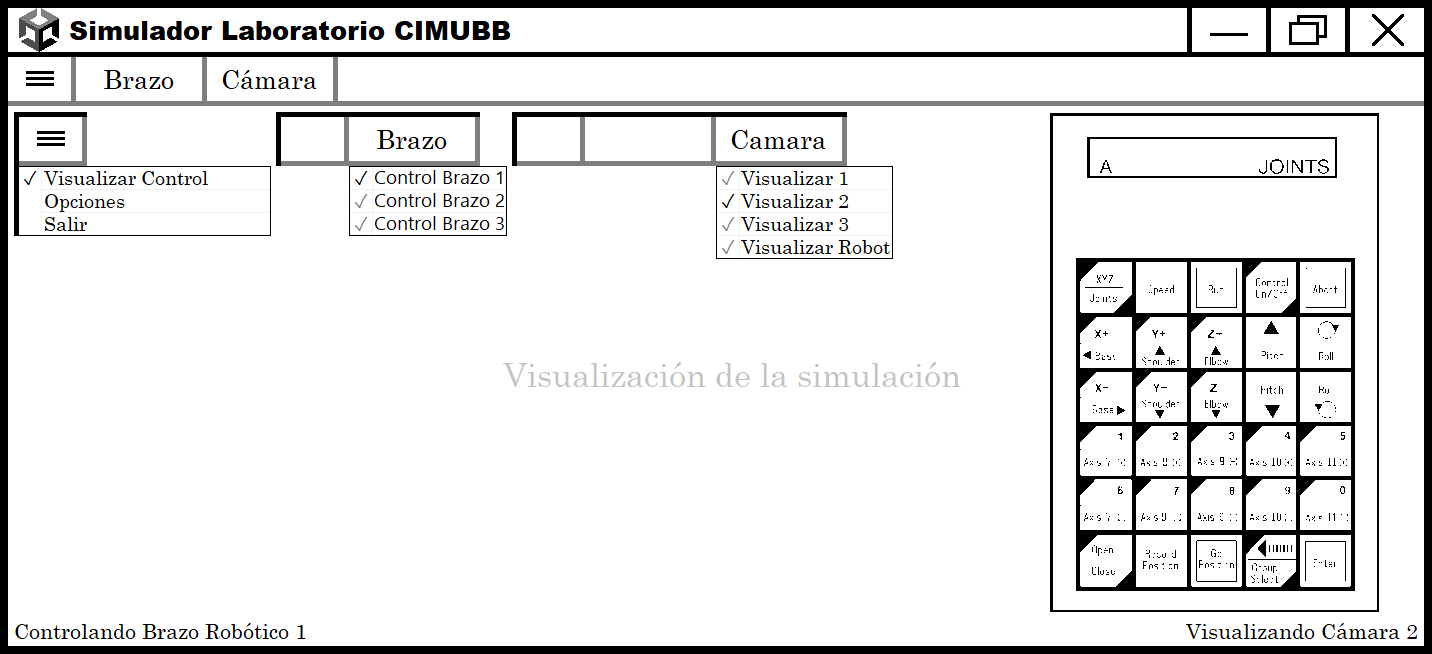
\includegraphics[width=16cm]{figures/Mockup.png}
\caption{Mockup}
\label{fig:Mockup}
\end{figure}
\clearpage

\begin{figure}[ht]
\centering
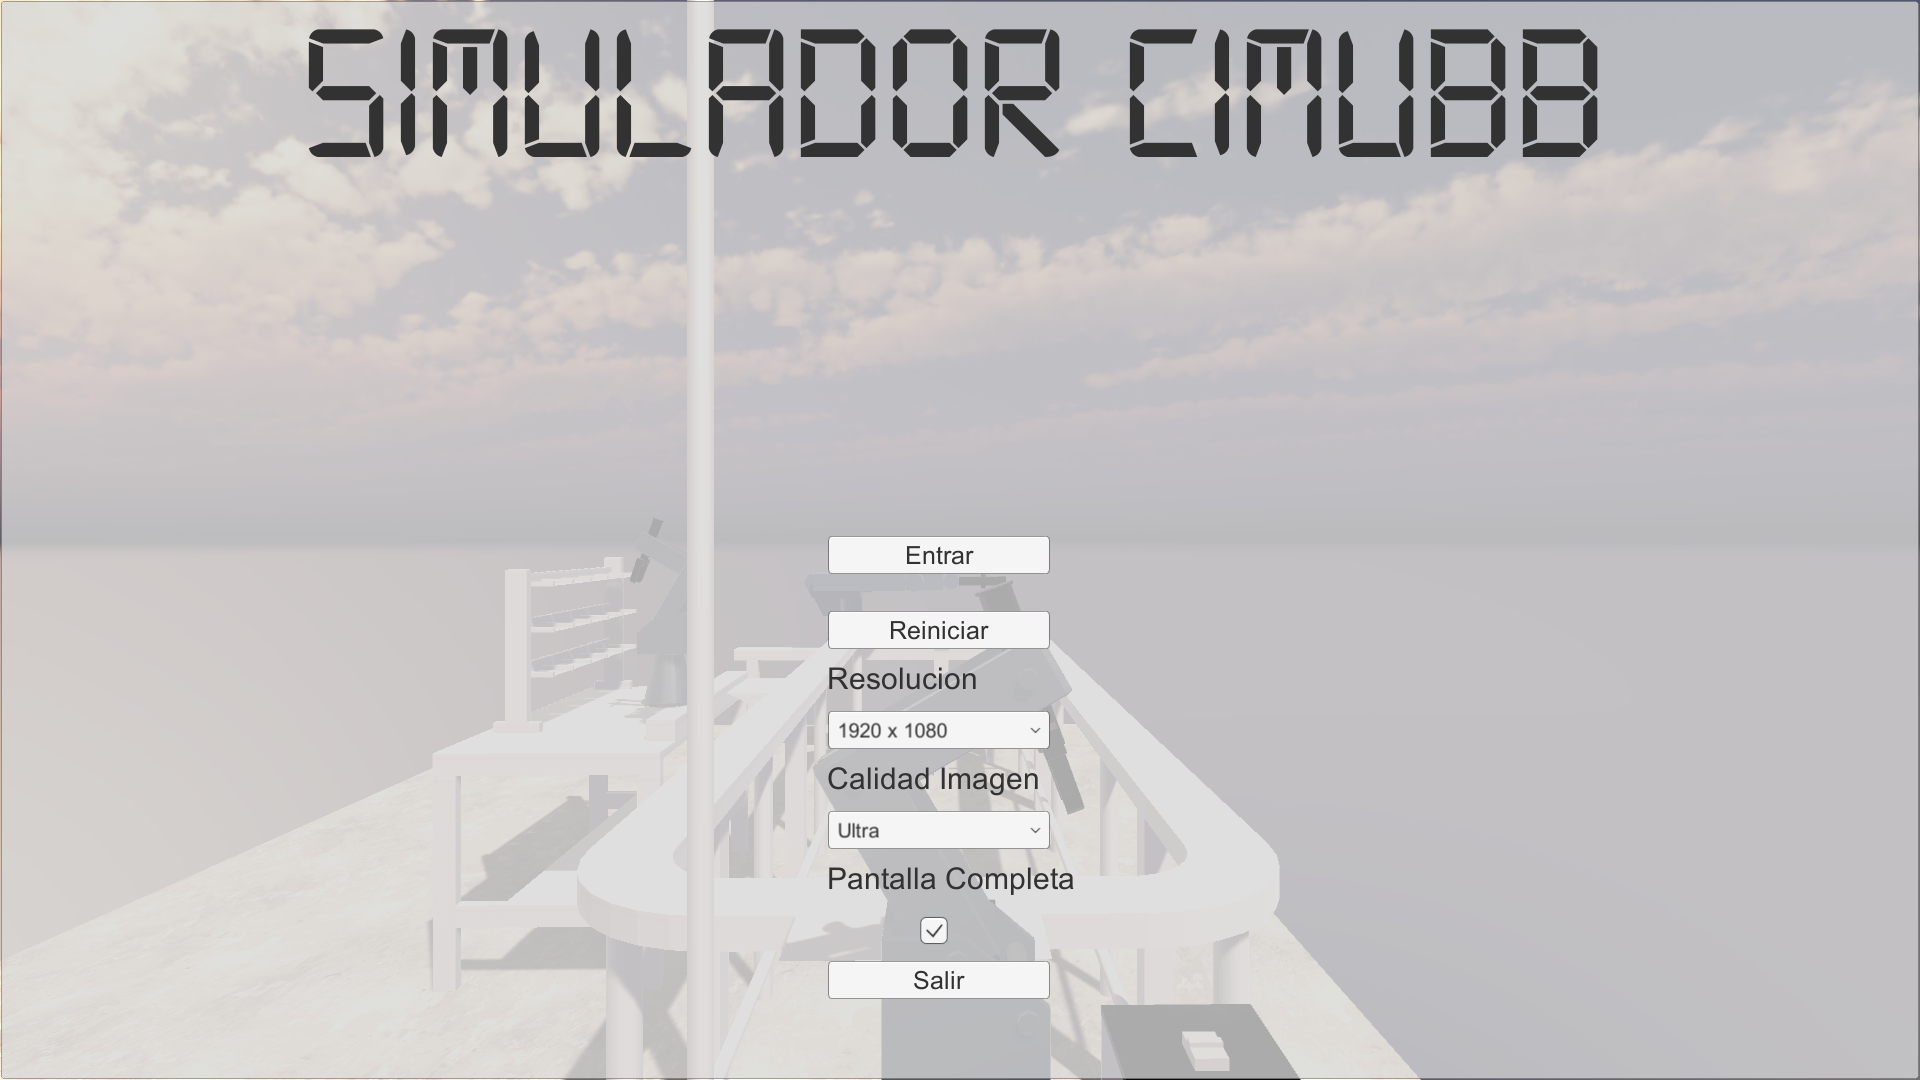
\includegraphics[width=16cm]{figures/menu.png}
\caption{Menu Principal Simulación}
\label{fig:menu}
\end{figure}

Las distintas opciones que se muestran en la Figura ~\ref{fig:menu} se detallaran a continuación
\begin{itemize}
\item Entrar: Permite entrar a la simulación.
\item Reiniciar: Permite reiniciar la simulación, volviendo a la posición original.
\item Resolución: Permite cambiar la resolución del programa, esto permite adaptarse a diferentes resoluciones o utilizar menos recursos.
\item Calidad Imagen: Permite cambiar la calidad visual de la simulación, esto permite adaptarse a cualquier equipo ya tenga buenos recursos o no.
\item Pantalla Completa: Permite que el programa funcione en pantalla completa o en modo ventana,
\item Salir: Permite salir de la aplicación.
\end{itemize}

\clearpage
\begin{figure}[ht]
\centering
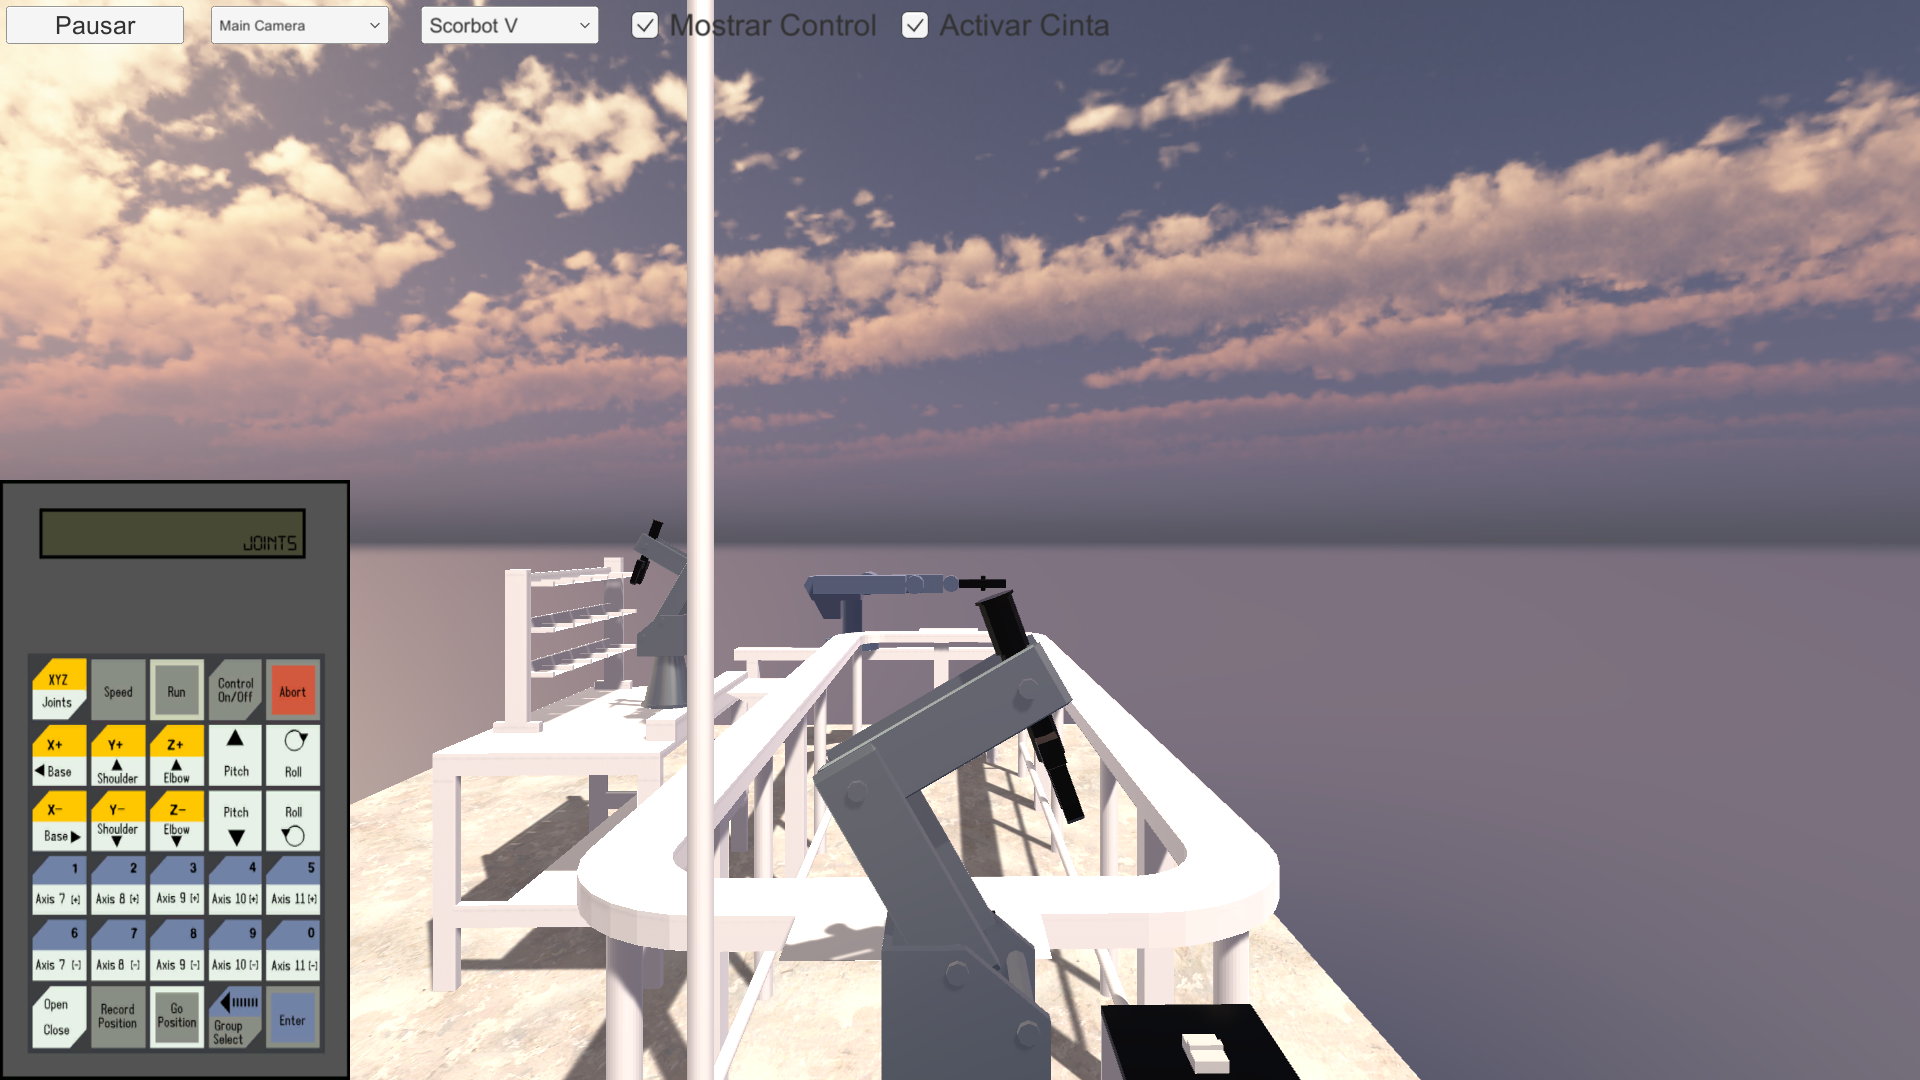
\includegraphics[width=16cm]{figures/simulacion.png}
\caption{Interfaz dentro de la Simulación}
\label{fig:interfaz}
\end{figure}


Las distintas opciones que se muestran en la Figura ~\ref{fig:interfaz} se detallaran a continuación
\begin{itemize}
\item Pausar: Permite pausar la simulación y volver al menu.
\item Lista Cámaras: Permite cambiar la perspectiva del usuario.
\item Lista Brazos Robóticos: Permite cambiar al robot controlado por el usuario.
\item Interruptor Mostrar Control: Permite cambiar la visibilidad de la botonera.
\item Interruptor Activar Cinta: Permite cambiar el estado de la cinta transportadora.
\item Botonera: Realiza las operaciones replicando el control de los brazos Scorbot reales.
\end{itemize}